\documentclass{beamer}
\usepackage{ctex, hyperref}
\usepackage[T1]{fontenc}
\usepackage{tabularx}
% other packages
\usepackage{latexsym,amsmath,xcolor,multicol,booktabs,calligra}
\usepackage{graphicx,pstricks,listings,stackengine}
:\usepackage{graphicx}
\usepackage{subfigure}
\author{王靖雄}
\title{本科生课程实验报告}
\subtitle{云原生微服务架构的研究与实践}
\institute{2020302111399}
\date{2023年6月5日}
\usepackage{whu}

% defs
\def\cmd#1{\texttt{\color{red}\footnotesize $\backslash$#1}}
\def\env#1{\texttt{\color{blue}\footnotesize #1}}
\definecolor{deepblue}{rgb}{0,0,0.5}
\definecolor{deepred}{rgb}{0.6,0,0}
\definecolor{deepgreen}{rgb}{0,0.5,0}
\definecolor{halfgray}{gray}{0.55}

\lstset{
    basicstyle=\ttfamily\small,
    keywordstyle=\bfseries\color{deepblue},
    emphstyle=\ttfamily\color{deepred},    % Custom highlighting style
    stringstyle=\color{deepgreen},
    numbers=left,
    numberstyle=\small\color{halfgray},
    rulesepcolor=\color{red!20!green!20!blue!20},
    frame=shadowbox,
}

\begin{document}

\kaishu
\begin{frame}
    \titlepage
    \begin{figure}[htpb]
        \begin{center}
            
\includegraphics[width=0.2\linewidth]{pic/whulogo.png}
        \end{center}
    \end{figure}
\end{frame}

\begin{frame}
    \tableofcontents[sectionstyle=show,subsectionstyle=show/shaded/hide,subsubsectionstyle=show/shaded/hide]
\end{frame}

\section{概述}
\begin{frame}{选题背景与实验目的}
	\begin{itemize}
		\item 云原生微服务架构的快速发展和应用,使之成为构建现代web应用的首选方法;
		\item Kubernetes作为容器编排平台,提供简化应用部署和管理,提供弹性和可伸缩性;
		\item 进一步探索在Kubernetes中配置和使用Kiali、Jaeger、Prometheus和Grafana等工具,实现服务网格的可视化、链路追踪、日志监控和健康状态监测。
		\item 使用Online Boutique示例应用,探索解决微服务挑战的服务网格框架,展示云原生微服务架构的最佳实践。
	\end{itemize}
\end{frame}

\begin{frame}{实验主要内容}
\begin{enumerate}
	\item 安装和配置Kubernetes集群环境;
	\item 部署Online Boutique应用到Kubernetes;
	\item 引入Istio服务网格框架,提升微服务能力;
	\item 配置Kiali实现服务网格的可视化,特别地,使用流量追踪功能;
	\item 配置Jaeger实现分布式调用链追踪;
	\item 安装Prometheus和Grafana进行集群监控,特别地,使用Grafana监控故障注入;
\end{enumerate}
\end{frame}

\section{微服务部署与验证}
\begin{frame}{Kubernetes集群搭建}
\begin{tabular}{|l|l|l|}\hline\hline
	虚拟机hostname        & IP地址&含义              \\ \hline
	master&192.168.210.128&集群主节点\\ \hline
	node1&192.168.210.129& 集群从节点1\\ \hline
	node2&192.168.210.130& 集群从节点2\\ \hline\hline
\end{tabular}
\begin{figure}[htpb]
	\centering
	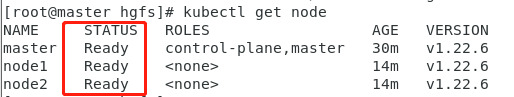
\includegraphics[width=1.0\linewidth]{pic/getnode.png}
	\caption{集群节点验证}
\end{figure}

\end{frame}

\begin{frame}{Kubernetes Dashboard部署}
\begin{figure}[htpb]
	\centering
	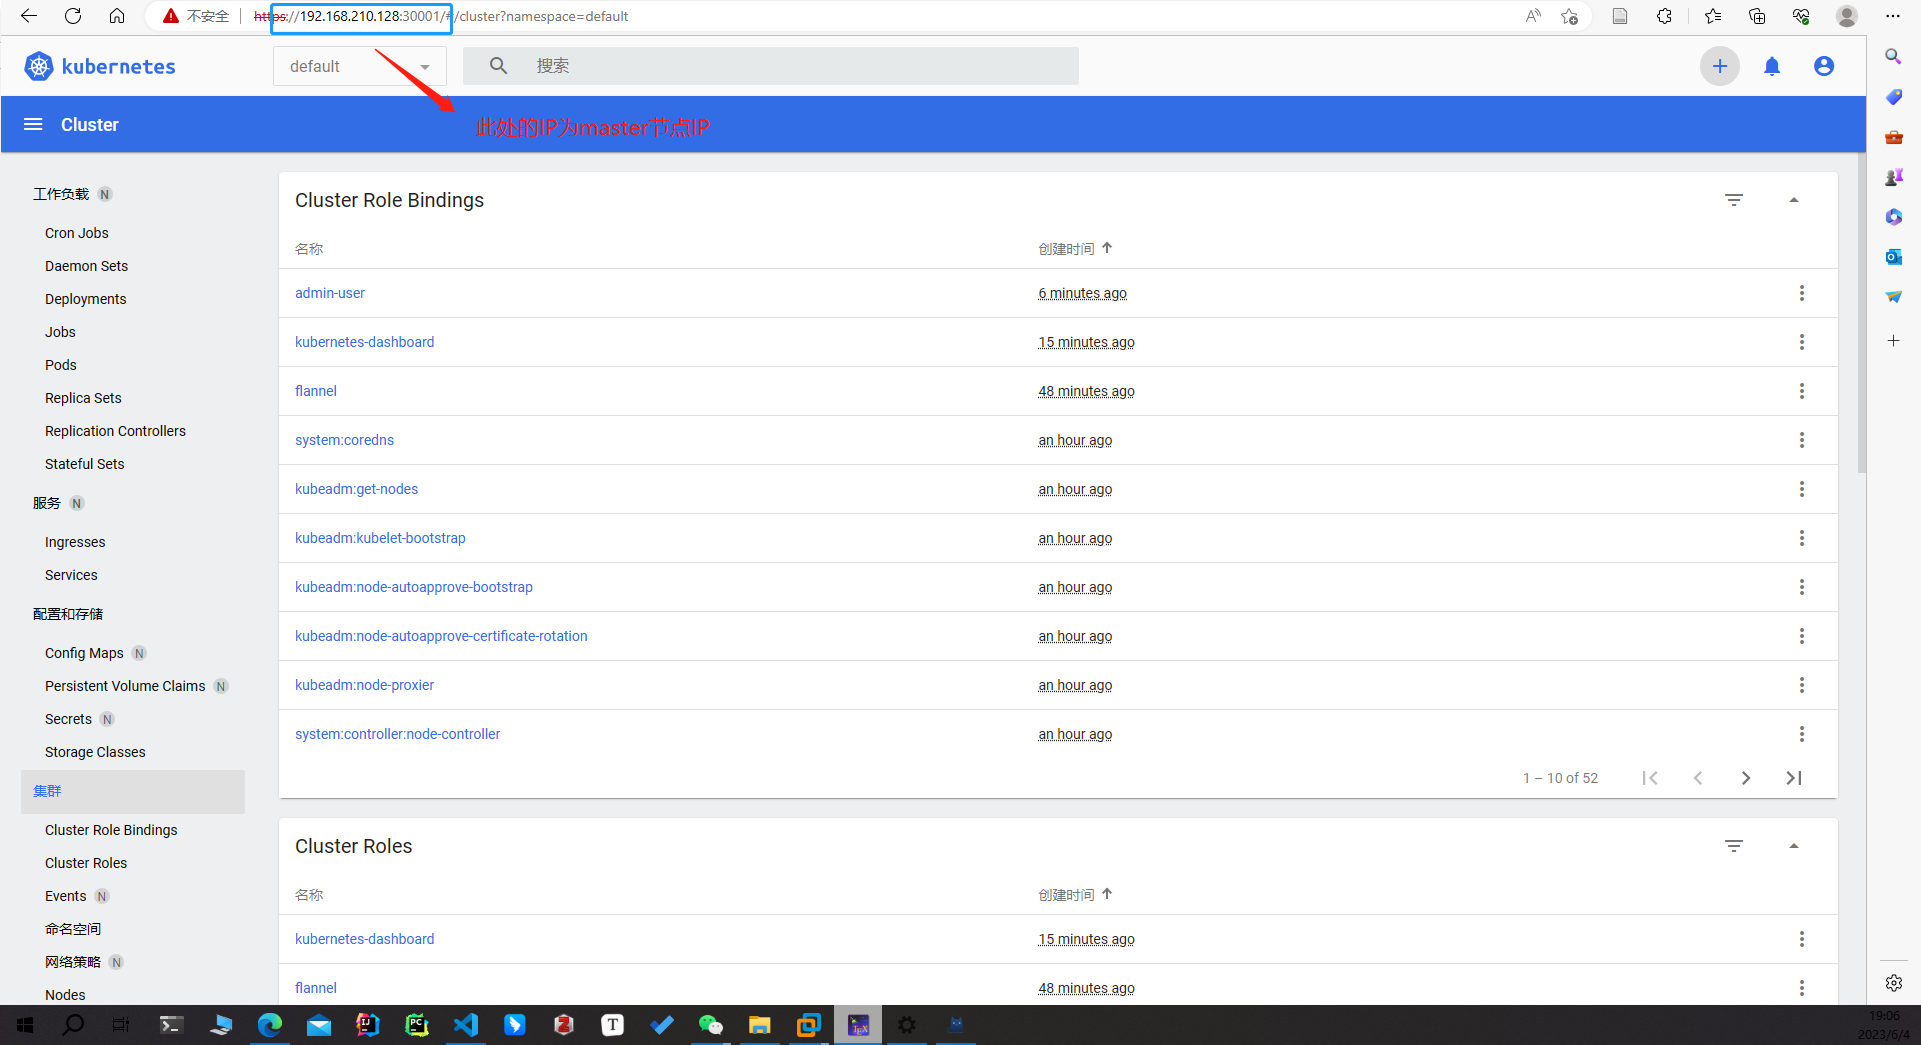
\includegraphics[width=0.9\linewidth]{pic/dashboard.png}
	\caption{Kubernetes Dashboard部署}
\end{figure}
\begin{itemize}
	\item IP: 192.168.210.128 Port:30001
\end{itemize}
\end{frame}

\section{Istio与Online-Boutique项目微服务部署}
\begin{frame}{单体架构与微服务架构}
	\begin{tabularx}{\textwidth} {X|X}
		\hline
		\textbf{单体架构缺陷} & \textbf{微服务架构优势} \\
		\hline
		系统启动慢,系统错误隔离性差、可用性差,系统可伸缩性差。扩容只能只对这个应用进行扩容,不能做到对某个功能点进行扩容,线上问题修复周期长。 & 微服务架构中,每个微服务专注于特定的业务功能,整体应用保持可控状态。启动速度快,对某个微服务进行修改只需要重新部署该服务即可。 \\
		\hline
	\end{tabularx}
	\begin{itemize}
		\item 通过微服务架构,我们可以充分利用其优势,使得开发和维护变得简单高效。同时,根据项目需求和团队特点,选择适合的技术工具和灵活扩展方式,为应用提供高度可定制的解决方案。
	\end{itemize}
\end{frame}
\begin{frame}{Online-Boutique模块分析}
	\begin{tabularx}{\textwidth}{|l|l|X|}
		\hline
		\textbf{服务} & \textbf{编程语言} & \textbf{描述} \\
		\hline	
		前端服务 & Go & HTTP服务器来提供网站 \\\hline
		购物车服务 & C\# & 将购物车存储在Redis \\\hline
		产品目录服务 & Go & 提供产品列表 \\\hline
		货币转换服务 & Node.js & 货币金额转换 \\\hline
		支付服务 & Node.js & 模拟进行扣款 \\\hline
		配送服务 & Go & 提供运费估算与商品运送\\\hline
		邮件服务 & Python & 发送订单确认邮件\\\hline
		结账服务 & Go & 协调支付、配送和邮件通知 \\\hline
		推荐服务 & Python & 推荐其他产品。 \\\hline
		广告服务 & Java & 提供文本广告。 \\\hline
		负载生成器 & Python/Locust & Locust负载生成器 \\
		\hline
	\end{tabularx}

\end{frame}
\begin{frame}{Online-Boutique微服务部署}
\begin{figure}[H]
	\centering
	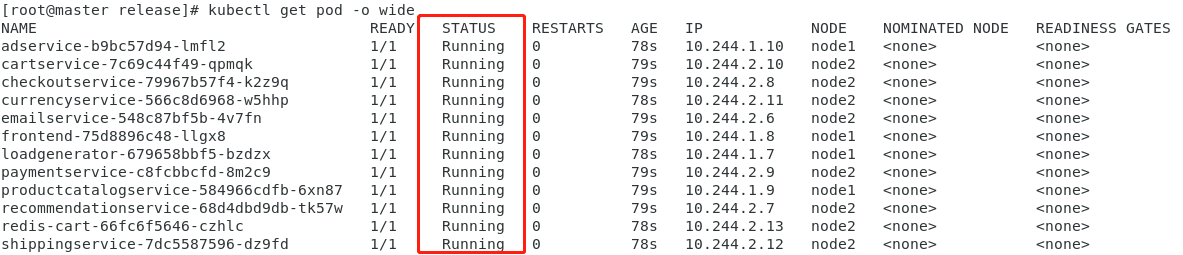
\includegraphics[width=1.0\textwidth]{pic/nodes.png}
	\caption{Online-Boutique各pod状态}
\end{figure}
\begin{itemize}
	\item 在 `istio-manifests` 目录中找到了 Istio 相关的 YAML 文件;
	\item 通过使用 `kubectl apply` 命令,创建 Istio 相关的资源,如 ServiceEntry、Gateway、VirtualService。
\end{itemize}
\end{frame}
\begin{frame}
	\begin{figure}[H]
		\centering
		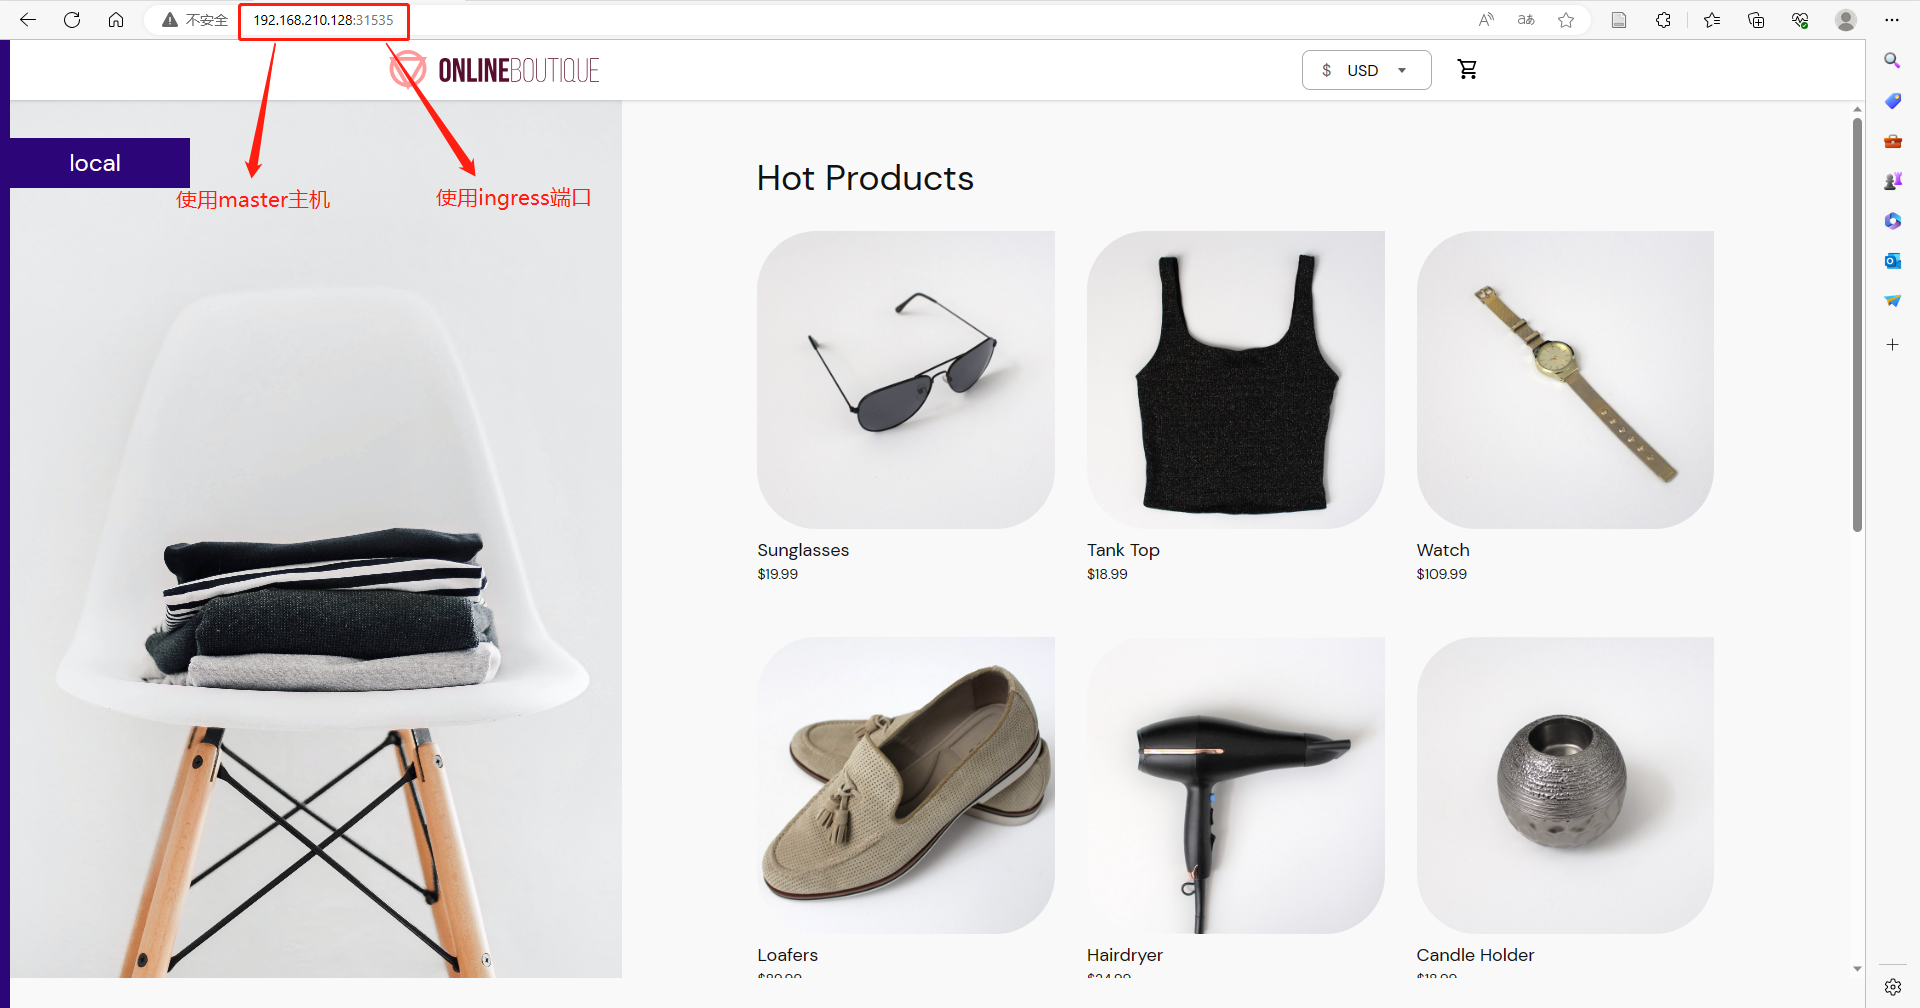
\includegraphics[width=1.0\textwidth]{pic/Online Boutique.png}
		\caption{Online Boutique前端界面,使用ingress入口网关访问}
	\end{figure}
\end{frame}
\begin{frame}
	\begin{figure}[H]
		\centering
		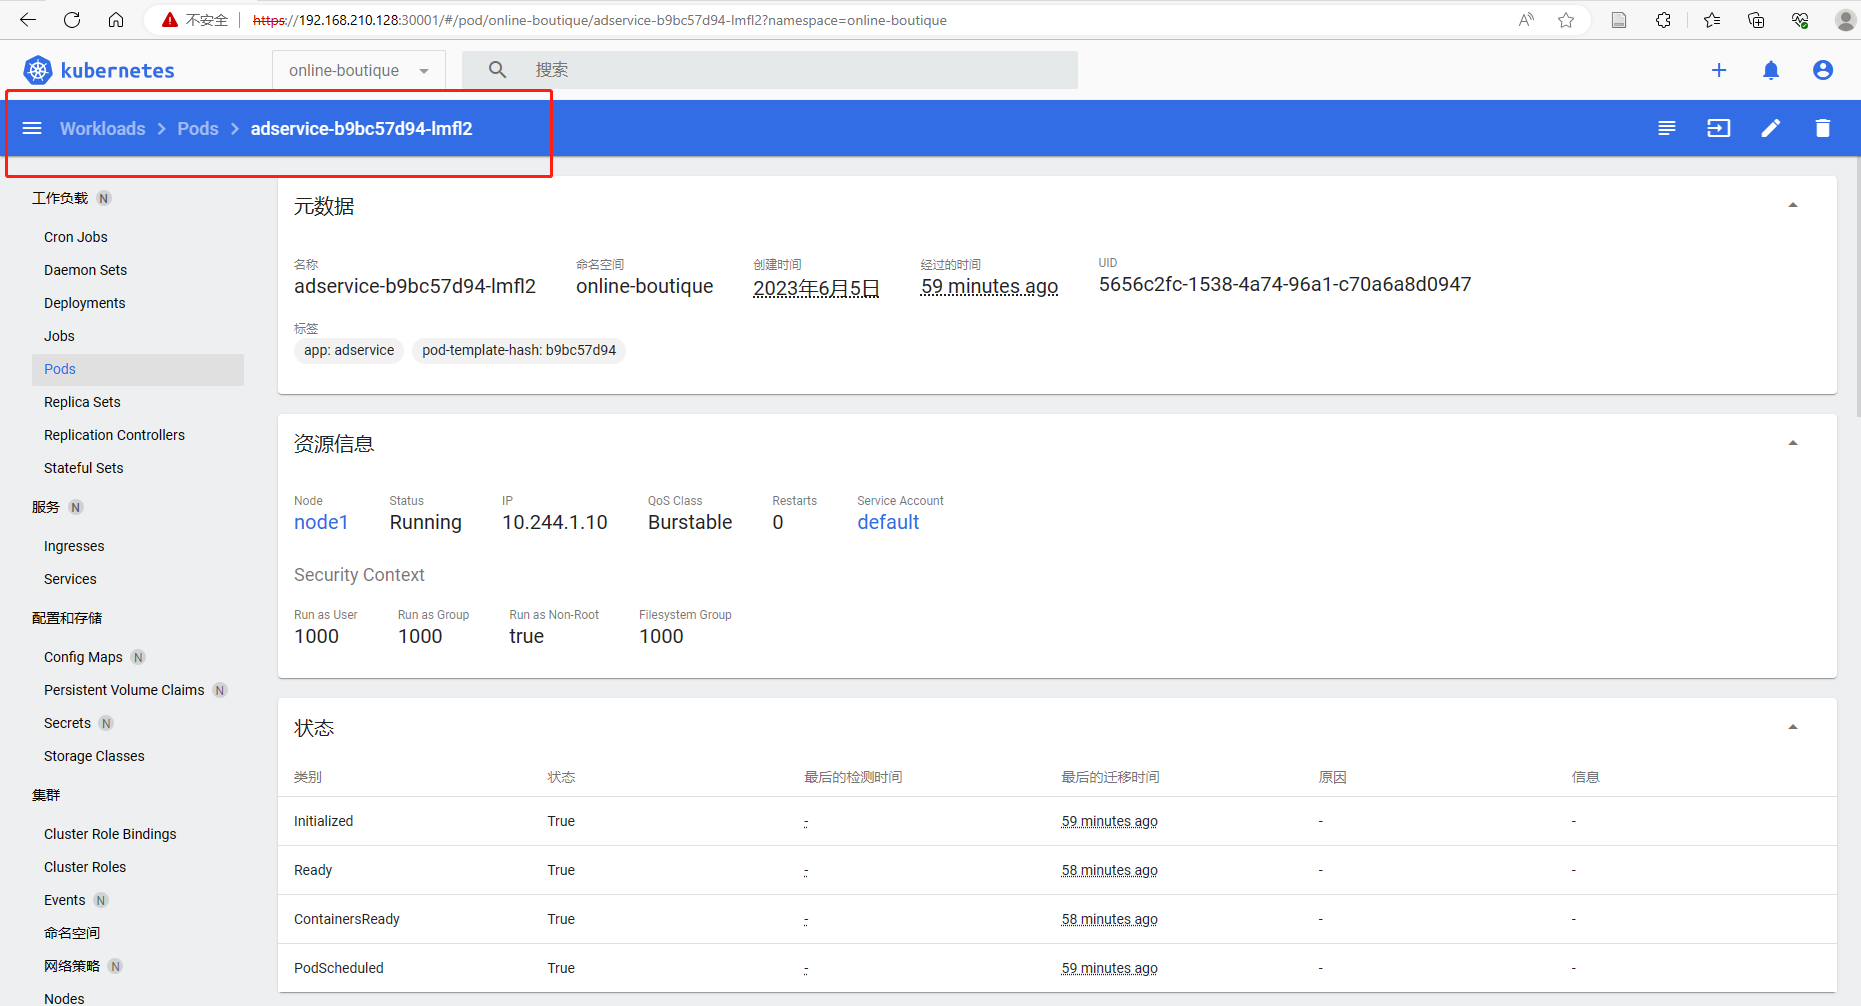
\includegraphics[width=1.0\textwidth]{pic/online boutique on dashboard.png}
		\caption{online boutique命名空间下的服务,以adservice为例}
	\end{figure}
\end{frame}
\section{服务治理与监控}
\begin{frame}{Prometheus 的配置与使用}
\begin{figure}[H]
	\centering
	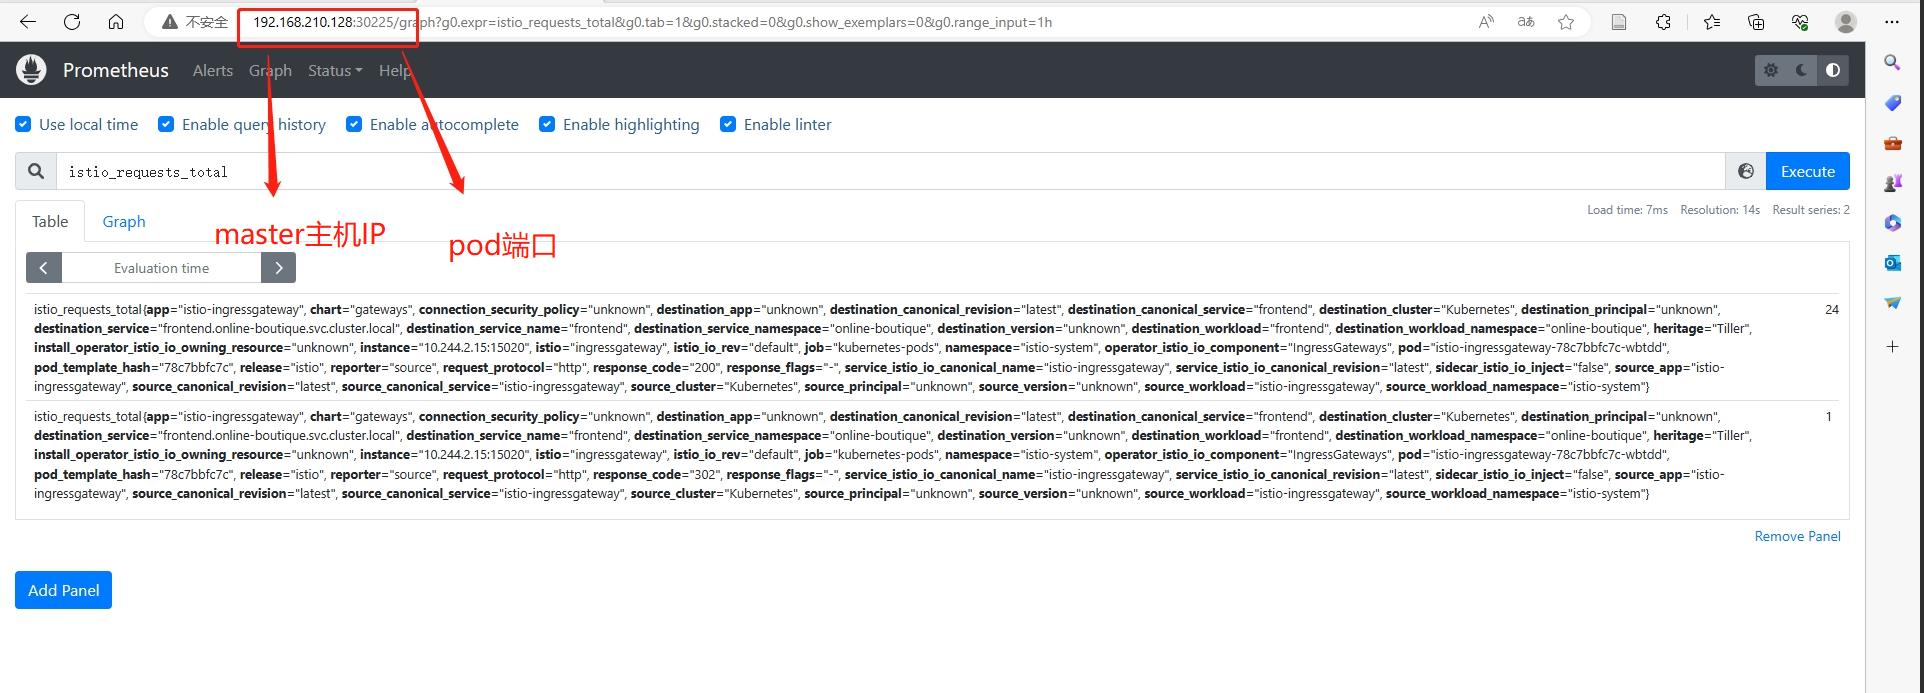
\includegraphics[width=1.0\textwidth]{pic/prometheus.png}
	\caption{}
\end{figure}
\end{frame}
\begin{frame}{Grafana的配置和使用}
\begin{figure}[H]
	\centering
	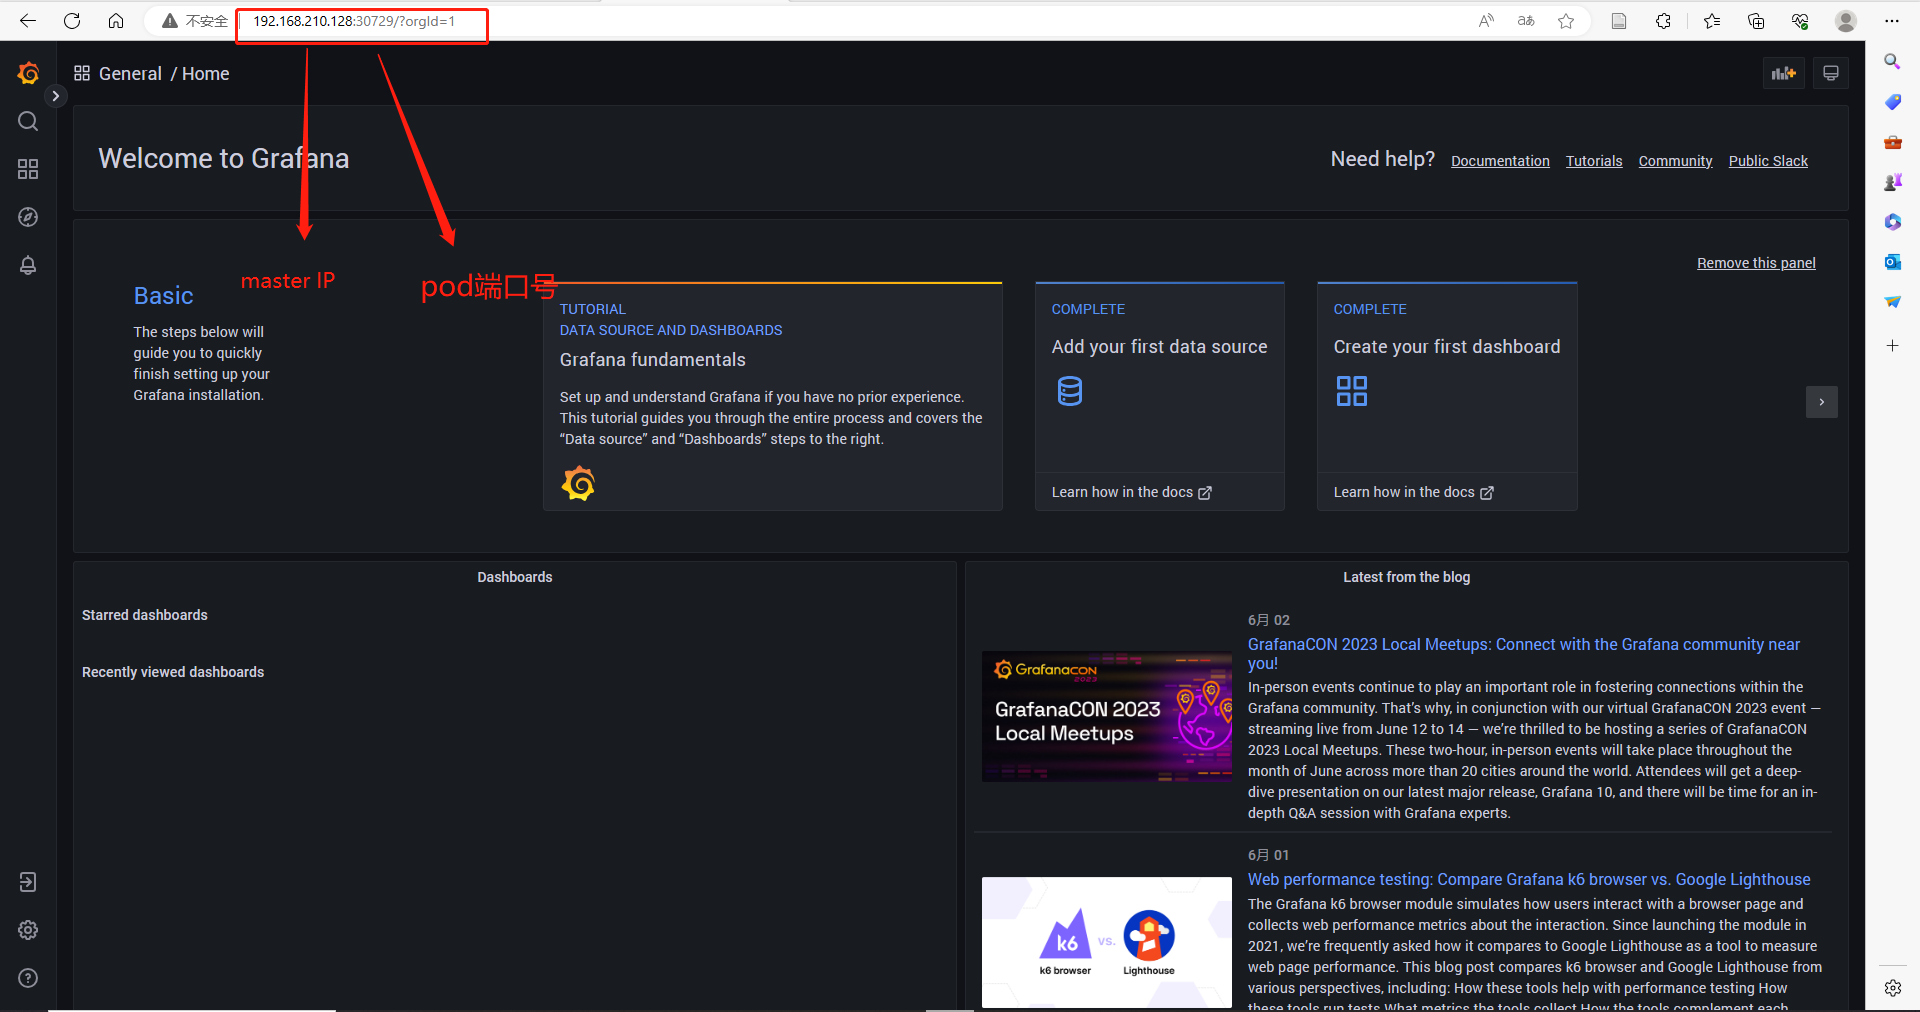
\includegraphics[width=1.0\textwidth]{pic/grafana.png}
	\caption{}
\end{figure}
\end{frame}
\begin{frame}{Grafana的各种Dashboard}
\begin{figure}[htbp]
	\centering
	\subfloat
	{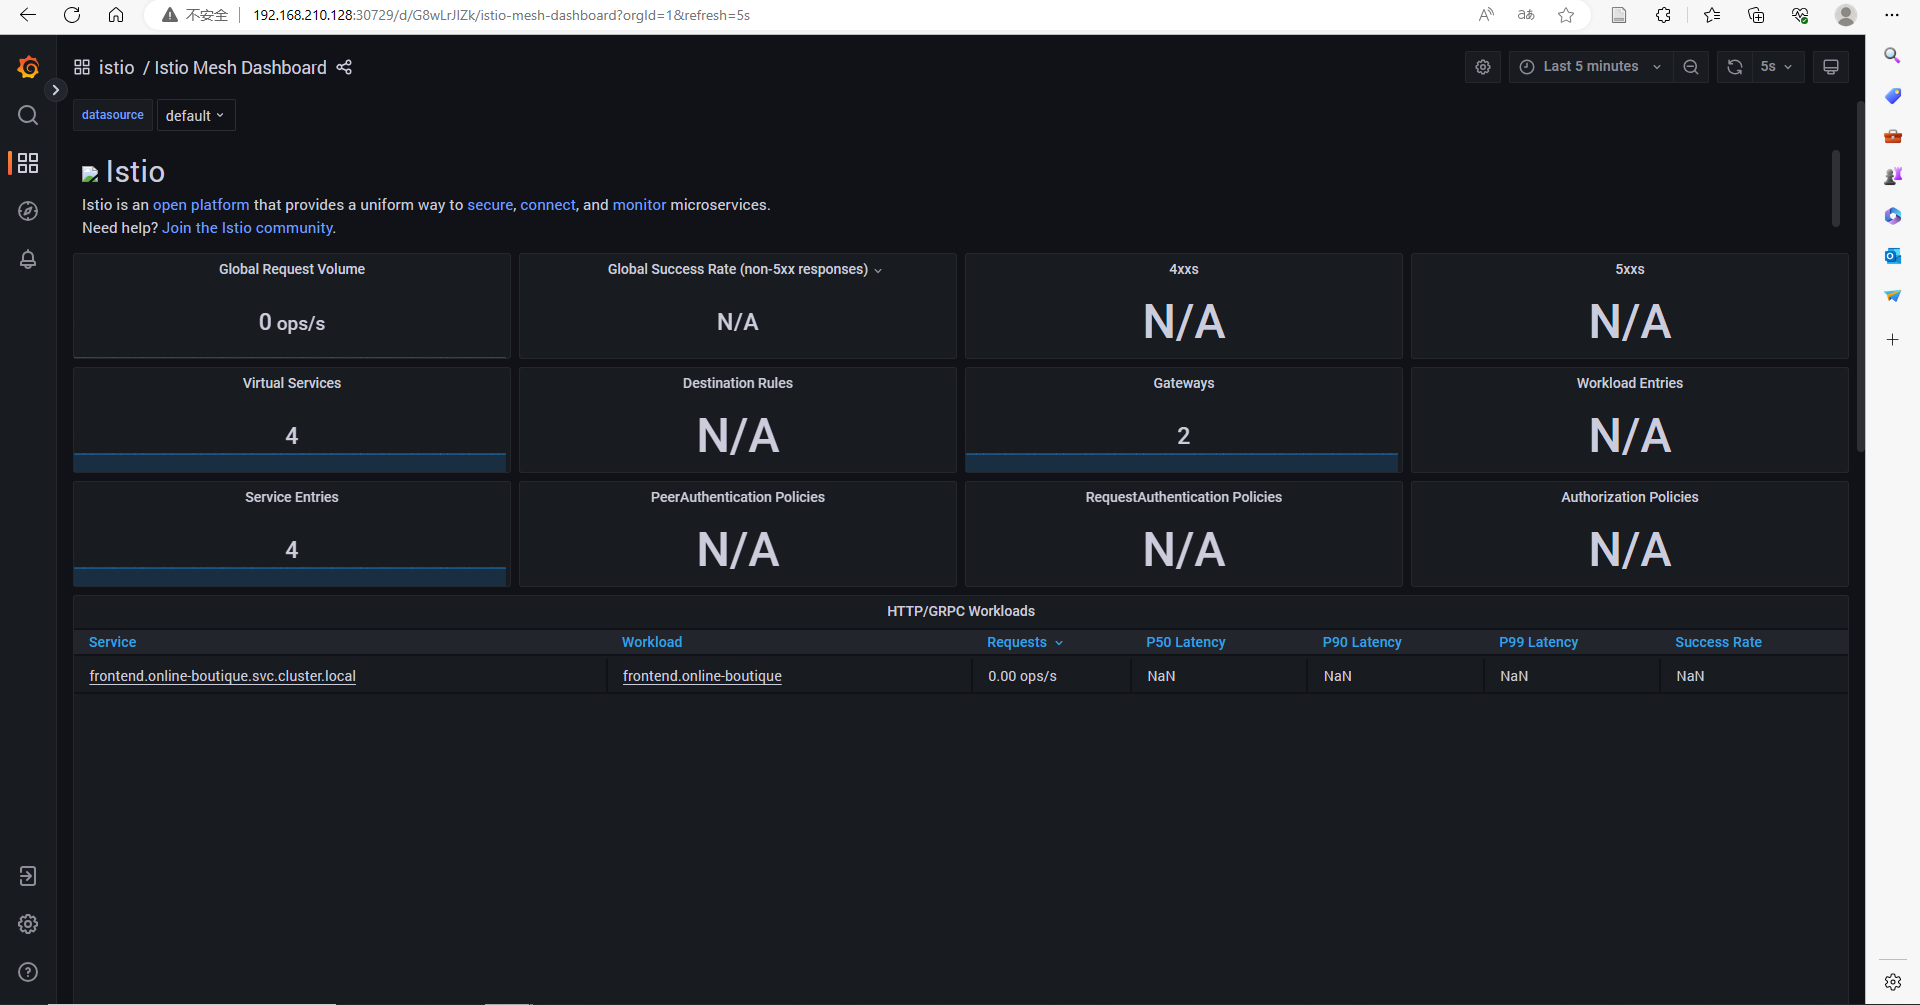
\includegraphics[width=0.4\textwidth]{pic/MD.png}
	\caption{Istio 网格仪表盘(Istio Mesh Dashboard)}}
	\subfloat
	{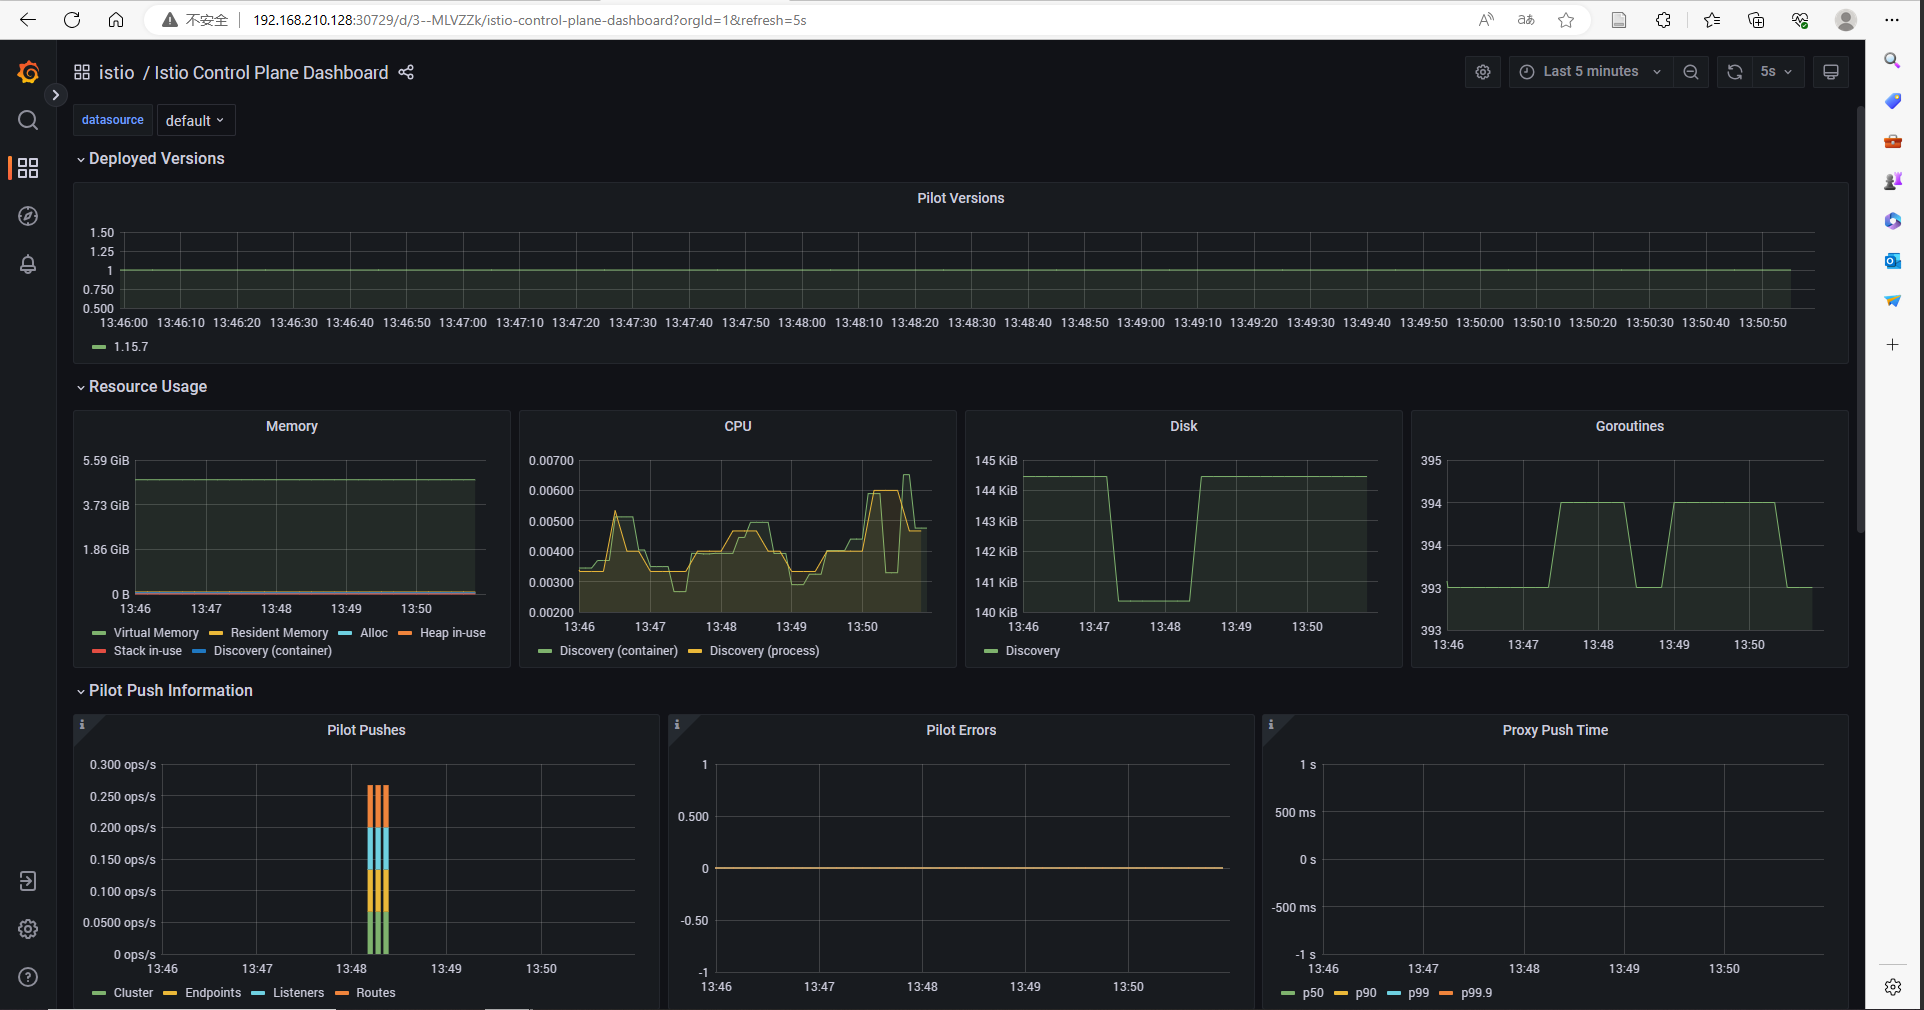
\includegraphics[width=0.4\textwidth]{pic/CPA}
	\caption{Istio 控制平面仪表盘(Istio Control Plane Dashboard)}}
\end{figure}
\end{frame}
\begin{frame}{Grafana的各种Dashboard}
	\begin{figure}[hdbp]
			\subfloat
		{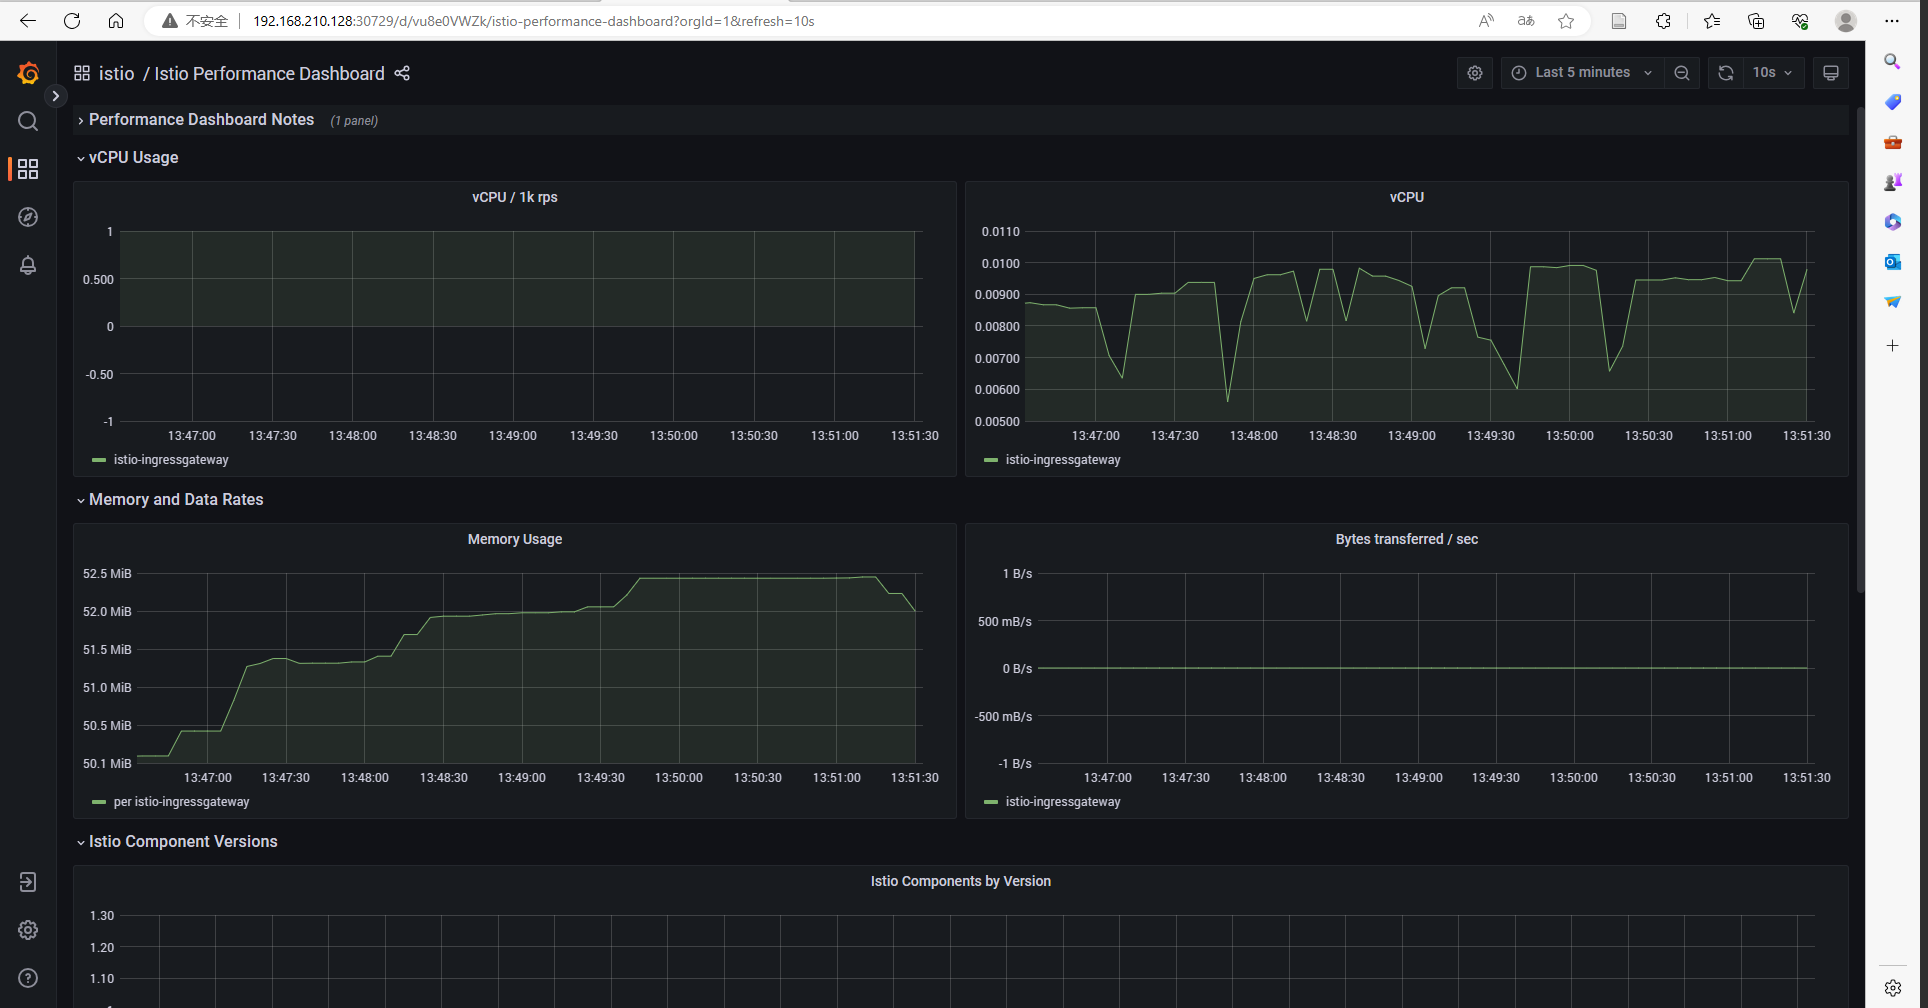
\includegraphics[width=0.4\textwidth]{pic/PD.png}
			\caption{Istio 性能仪表盘(Istio Performance Dashboard)}}
		\subfloat
		{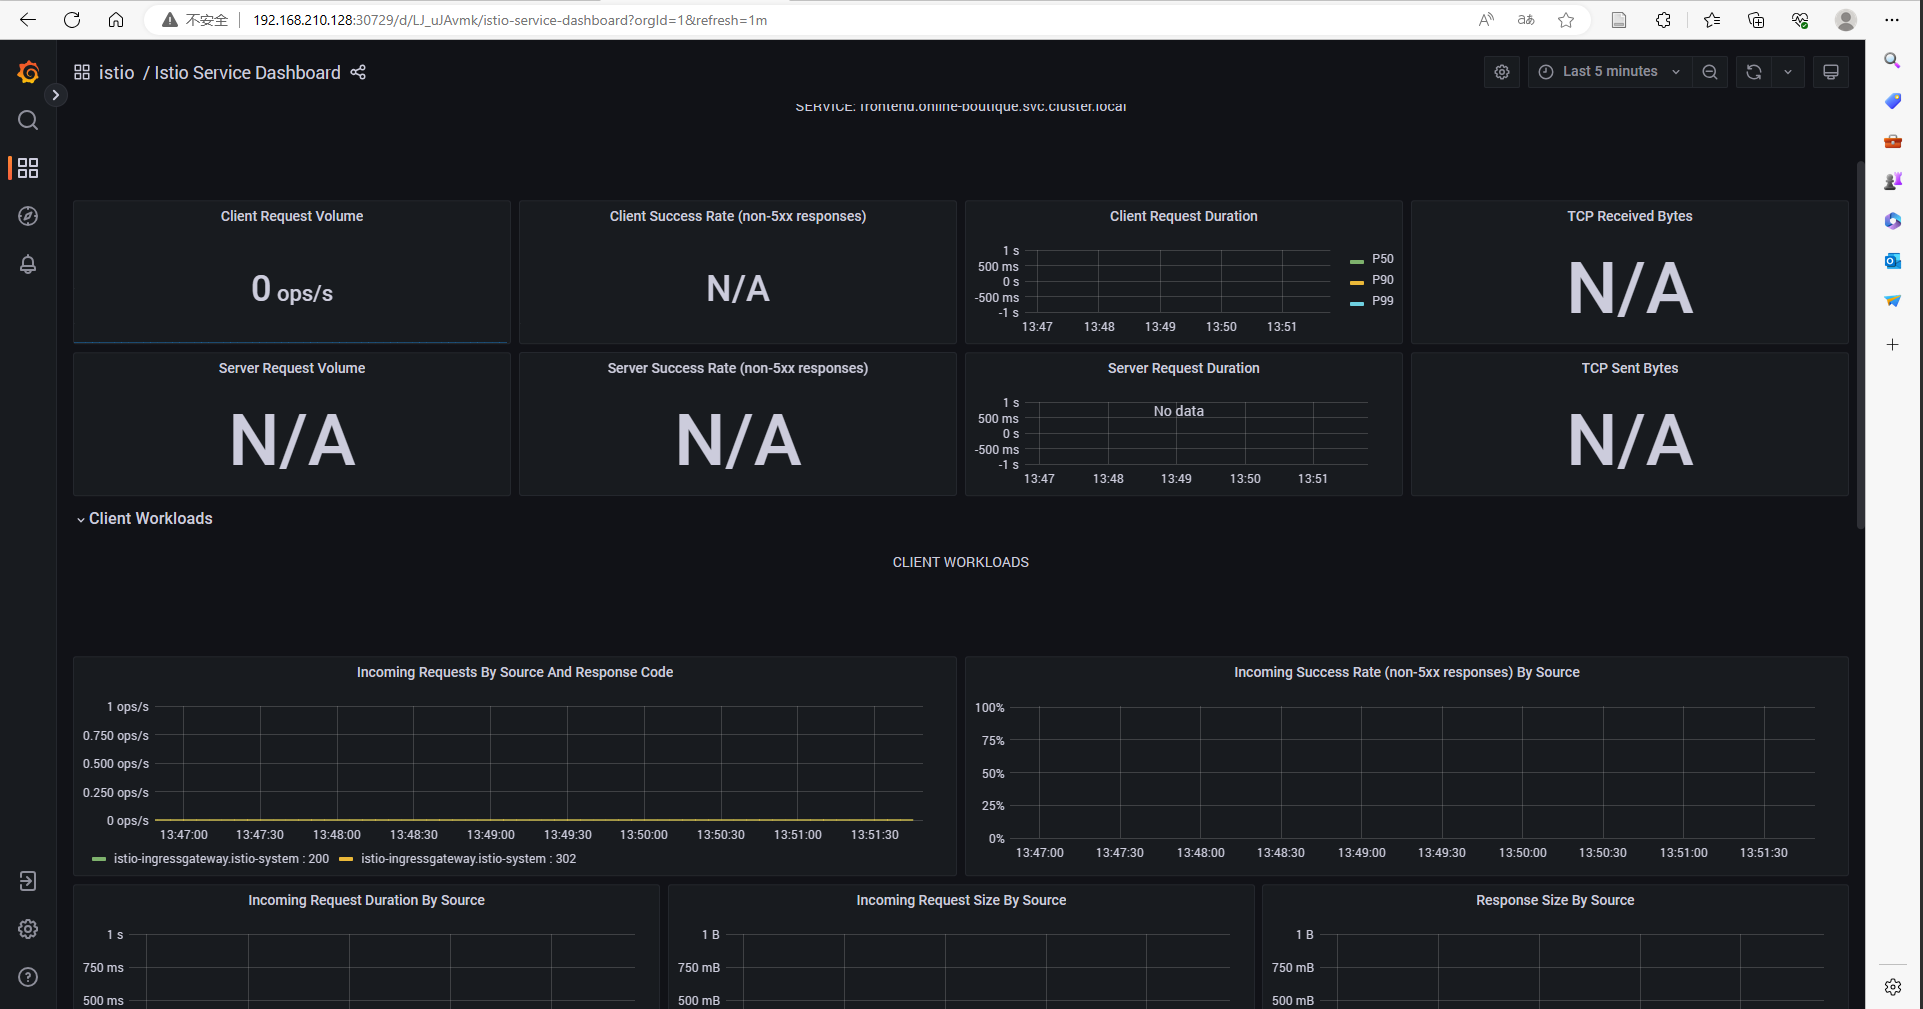
\includegraphics[width=0.4\textwidth]{pic/SD.png}
			\caption{Istio 服务仪表盘(Istio Service Dashboard)}}
	\end{figure}
\end{frame}

\begin{frame}{Kiali的配置和使用}
\begin{figure}[H]
	\centering
	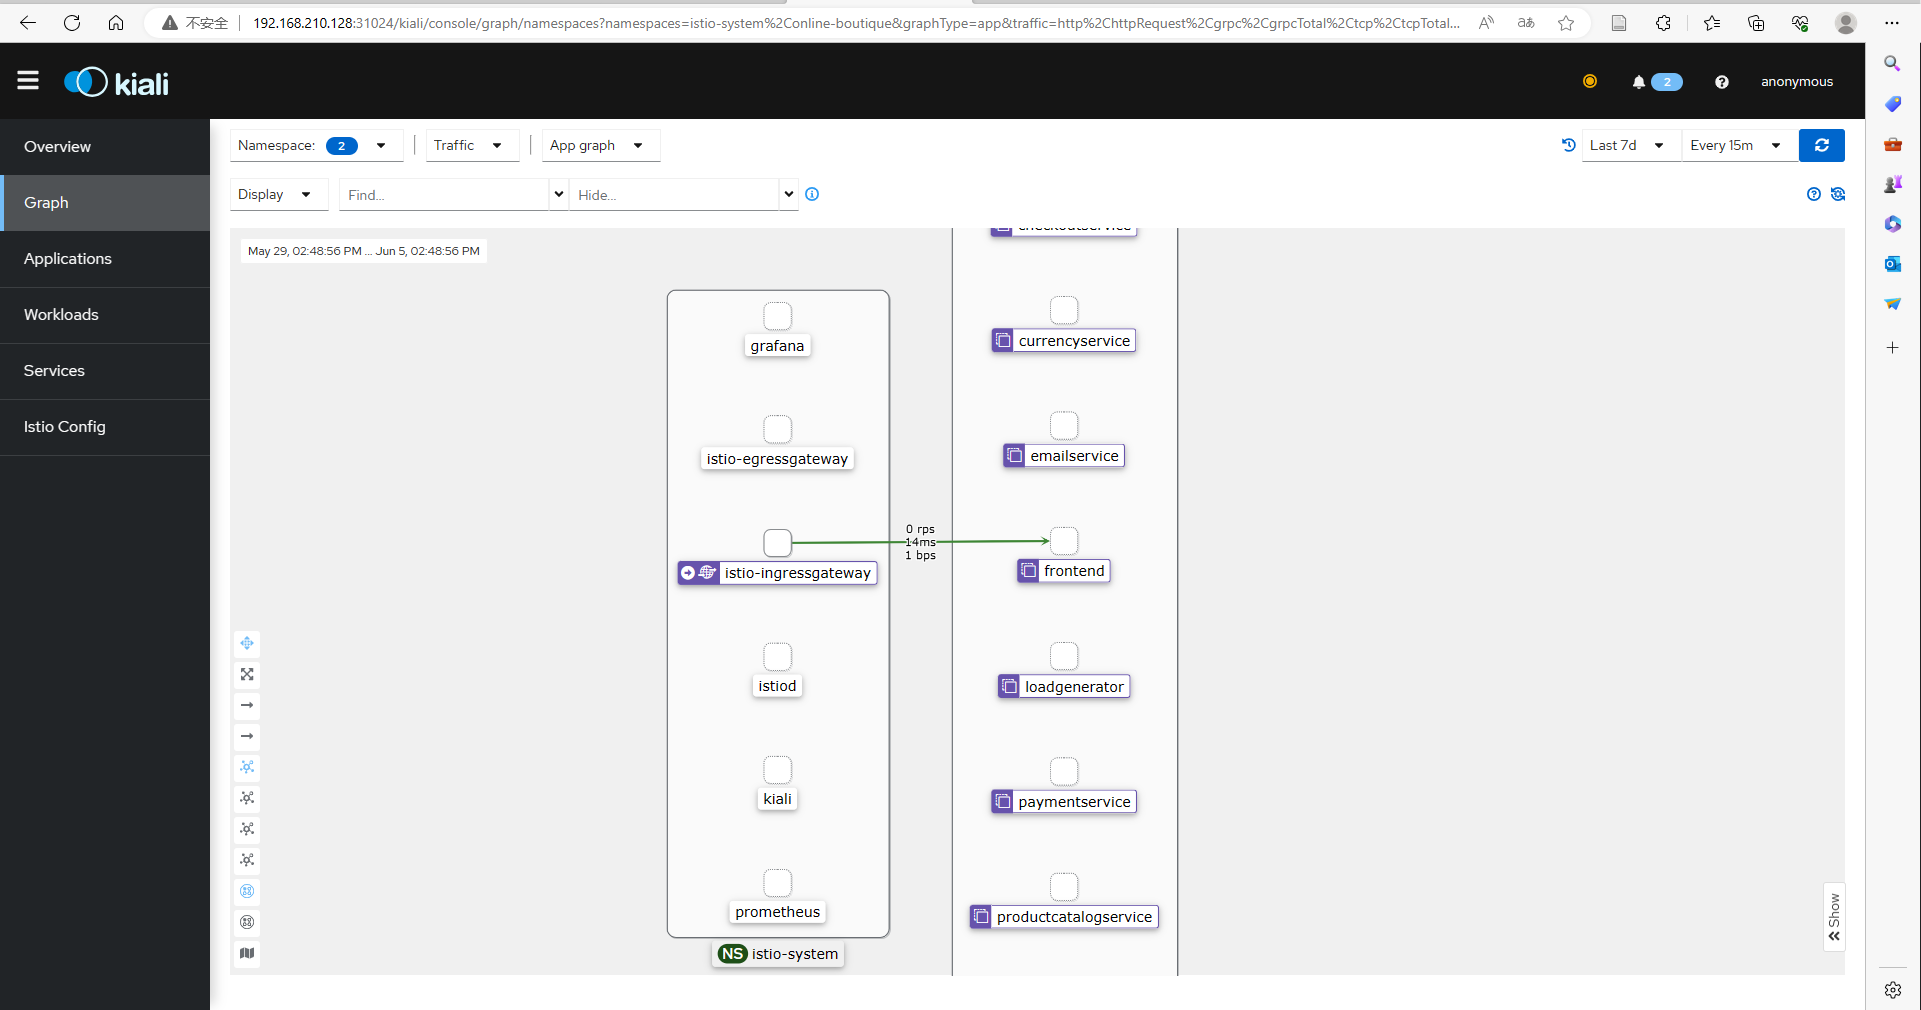
\includegraphics[width=1.0\textwidth]{pic/online-boutique-kiali.png}
	\caption{}
\end{figure}
\end{frame}
\begin{frame}{Jaeger的配置和使用}
\begin{figure}[H]
	\centering
	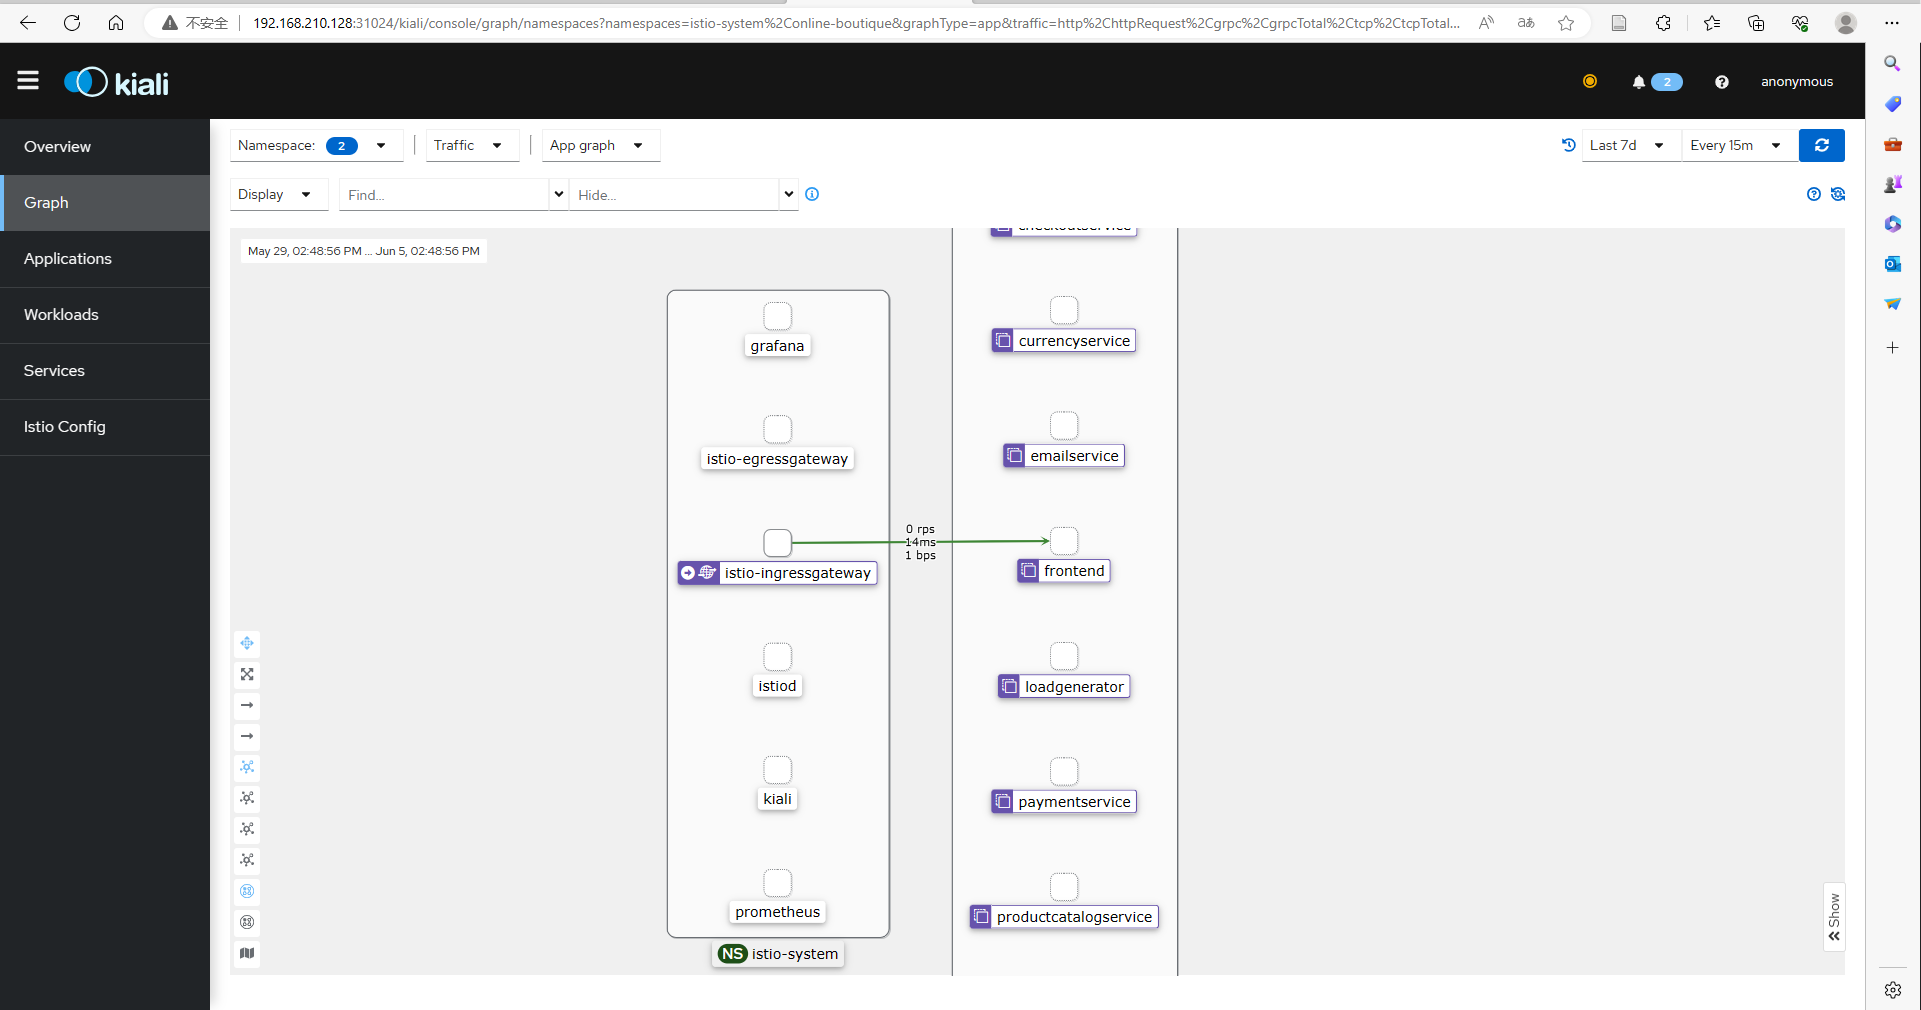
\includegraphics[width=1.0\textwidth]{pic/online-boutique-kiali.png}
	\caption{}
\end{figure}
\end{frame}

\section{使用Grafana监控故障注入}

\section{使用kiali监控流量}

\section{概述}
\begin{frame}{用Beamer很5高大上?}
    \begin{itemize}[<+-| alert@+>] % 当然,除了alert,手动在里面插 \pause 也行
        \item 大家都会\LaTeX{},好多学校都有自己的Beamer主题
        \item 中文支持请选择 Xe\LaTeX{} 编译选项
        \item 原 THU Beamer Github项目地址位于 \url{https://github.com/tuna/THU-Beamer-Theme}
        \item 本魔改 GitHub项目地址位于 \url{https://github.com/Xinchen-Fan/WHU-Beamer-Theme},如果有bug或者feature request可以去里面提issue
    \end{itemize}
\end{frame}


\section{研究现状}

\subsection{Beamer主题分类}

\begin{frame}
    \begin{itemize}
        \item 有一些 \LaTeX{} 自带的
        \item 有一些Tsinghua的
        \item 本模板来源自 \newline \url{https://www.latexstudio.net/archives/4051.html}
        \item 但是最初的 \href{http://far.tooold.cn/post/latex/beamertsinghua}{\color{purple}{link}} \cite{origin}已经失效了
        \item 这是THU原作者大佬在16-17年做的一些ppt:\href{https://github.com/Trinkle23897/oi_slides}{\color{purple}{戳我}}
    \end{itemize}
\end{frame}


\section{研究内容}

\subsection{美化主题}

\begin{frame}{这一份主题与原始的THU Beamer Theme区别在于}
    \begin{itemize}
        \item 顶栏的小点变成一行而不是多行
        \item 中文采用楷书
        \item 剩下我改了啥我也忘了……我16年魔改的,都四年过去了(x
        \item 更多该模板的功能可以参考 \url{https://www.latexstudio.net/archives/4051.html}
        \item 下面列举出了一些Beamer的用法,部分节选自 \url{https://tuna.moe/event/2018/latex/}
    \end{itemize}
\end{frame}

\subsection{如何更好地做Beamer}

\begin{frame}{Why Beamer}
    \begin{itemize}
        \item \LaTeX 广泛用于学术界,期刊会议论文模板
    \end{itemize}
    \begin{table}[h]
        \centering
        \begin{tabular}{c|c}
            Microsoft\textsuperscript{\textregistered}  Word & \LaTeX \\
            \hline
            文字处理工具 & 专业排版软件 \\
            容易上手,简单直观 & 容易上手 \\
            所见即所得 & 所见即所想,所想即所得 \\
            高级功能不易掌握 & 进阶难,但一般用不到 \\
            处理长文档需要丰富经验 & 和短文档处理基本无异 \\
            花费大量时间调格式 & 无需担心格式,专心作者内容 \\
            公式排版差强人意 & 尤其擅长公式排版 \\
            二进制格式,兼容性差 & 文本文件,易读、稳定 \\
            付费商业许可 & 自由免费使用 \\
        \end{tabular}
    \end{table}
\end{frame}

\begin{frame}{排版举例}
    \begin{exampleblock}{无编号公式} % 加 * 
        \begin{equation*}
            J(\theta) = \mathbb{E}_{\pi_\theta}[G_t] = \sum_{s\in\mathcal{S}} d^\pi (s)V^\pi(s)=\sum_{s\in\mathcal{S}} d^\pi(s)\sum_{a\in\mathcal{A}}\pi_\theta(a|s)Q^\pi(s,a)
        \end{equation*}
    \end{exampleblock}
    \begin{exampleblock}{多行多列公式\footnote{如果公式中有文字出现,请用 $\backslash$mathrm\{\} 或者 $\backslash$text\{\} 包含,不然就会变成 $clip$,在公式里看起来比 $\mathrm{clip}$ 丑非常多。}}
        % 使用 & 分隔
        \begin{align}
            Q_\mathrm{target}&=r+\gamma Q^\pi(s^\prime, \pi_\theta(s^\prime)+\epsilon)\\
            \epsilon&\sim\mathrm{clip}(\mathcal{N}(0, \sigma), -c, c)\nonumber
        \end{align}
    \end{exampleblock}
\end{frame}

\begin{frame}
    \begin{exampleblock}{编号多行公式}
        % Taken from Mathmode.tex
        \begin{multline}
            A=\lim_{n\rightarrow\infty}\Delta x\left(a^{2}+\left(a^{2}+2a\Delta x+\left(\Delta x\right)^{2}\right)\right.\label{eq:reset}\\
            +\left(a^{2}+2\cdot2a\Delta x+2^{2}\left(\Delta x\right)^{2}\right)\\
            +\left(a^{2}+2\cdot3a\Delta x+3^{2}\left(\Delta x\right)^{2}\right)\\
            +\ldots\\
            \left.+\left(a^{2}+2\cdot(n-1)a\Delta x+(n-1)^{2}\left(\Delta x\right)^{2}\right)\right)\\
            =\frac{1}{3}\left(b^{3}-a^{3}\right)
        \end{multline}
    \end{exampleblock}
\end{frame}

\begin{frame}{图形与分栏}
    % From thuthesis user guide.
    \begin{minipage}[c]{0.3\linewidth}
        \psset{unit=0.8cm}
        \begin{pspicture}(-1.75,-3)(3.25,4)
            \psline[linewidth=0.25pt](0,0)(0,4)
            \rput[tl]{0}(0.2,2){$\vec e_z$}
            \rput[tr]{0}(-0.9,1.4){$\vec e$}
            \rput[tl]{0}(2.8,-1.1){$\vec C_{ptm{ext}}$}
            \rput[br]{0}(-0.3,2.1){$\theta$}
            \rput{25}(0,0){%
            \psframe[fillstyle=solid,fillcolor=lightgray,linewidth=.8pt](-0.1,-3.2)(0.1,0)}
            \rput{25}(0,0){%
            \psellipse[fillstyle=solid,fillcolor=yellow,linewidth=3pt](0,0)(1.5,0.5)}
            \rput{25}(0,0){%
            \psframe[fillstyle=solid,fillcolor=lightgray,linewidth=.8pt](-0.1,0)(0.1,3.2)}
            \rput{25}(0,0){\psline[linecolor=red,linewidth=1.5pt]{->}(0,0)(0.,2)}
%           \psRotation{0}(0,3.5){$\dot\phi$}
%           \psRotation{25}(-1.2,2.6){$\dot\psi$}
            \psline[linecolor=red,linewidth=1.25pt]{->}(0,0)(0,2)
            \psline[linecolor=red,linewidth=1.25pt]{->}(0,0)(3,-1)
            \psline[linecolor=red,linewidth=1.25pt]{->}(0,0)(2.85,-0.95)
            \psarc{->}{2.1}{90}{112.5}
            \rput[bl](.1,.01){C}
        \end{pspicture}
    \end{minipage}\hspace{1cm}
    \begin{minipage}{0.5\linewidth}
        \medskip
        %\hspace{2cm}
        \begin{figure}[h]
            \centering
            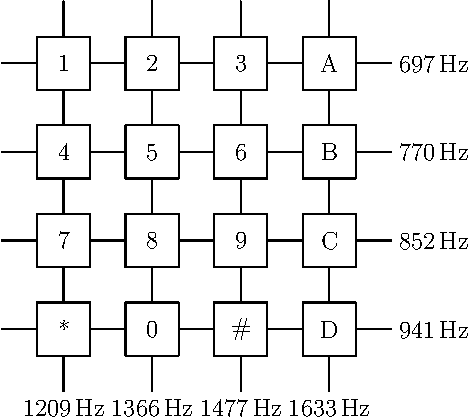
\includegraphics[height=.4\textheight]{pic/dtmf.pdf}
        \end{figure}
    \end{minipage}
\end{frame}

\begin{frame}[fragile]{\LaTeX{} 常用命令}
    \begin{exampleblock}{命令}
        \centering
        \footnotesize
        \begin{tabular}{llll}
            \cmd{chapter} & \cmd{section} & \cmd{subsection} & \cmd{paragraph} \\
            章 & 节 & 小节 & 带题头段落 \\\hline
            \cmd{centering} & \cmd{emph} & \cmd{verb} & \cmd{url} \\
            居中对齐 & 强调 & 原样输出 & 超链接 \\\hline
            \cmd{footnote} & \cmd{item} & \cmd{caption} & \cmd{includegraphics} \\
            脚注 & 列表条目 & 标题 & 插入图片 \\\hline
            \cmd{label} & \cmd{cite} & \cmd{ref} \\
            标号 & 引用参考文献 & 引用图表公式等\\\hline
        \end{tabular}
    \end{exampleblock}
    \begin{exampleblock}{环境}
        \centering
        \footnotesize
        \begin{tabular}{lll}
            \env{table} & \env{figure} & \env{equation}\\
            表格 & 图片 & 公式 \\\hline
            \env{itemize} & \env{enumerate} & \env{description}\\
            无编号列表 & 编号列表 & 描述 \\\hline
        \end{tabular}
    \end{exampleblock}
\end{frame}

\begin{frame}[fragile]{\LaTeX{} 环境命令举例}
    \begin{minipage}{0.5\linewidth}
\begin{lstlisting}[language=TeX]
\begin{itemize}
  \item A \item B
  \item C
  \begin{itemize}
    \item C-1
  \end{itemize}
\end{itemize}
\end{lstlisting}
    \end{minipage}\hspace{1cm}
    \begin{minipage}{0.3\linewidth}
        \begin{itemize}
            \item A
            \item B
            \item C
            \begin{itemize}
                \item C-1
            \end{itemize}
        \end{itemize}
    \end{minipage}
    \medskip
    \pause
    \begin{minipage}{0.5\linewidth}
\begin{lstlisting}[language=TeX]
\begin{enumerate}
  \item 巨佬 \item 大佬
  \item 萌新
  \begin{itemize}
    \item[n+e] 瑟瑟发抖
  \end{itemize}
\end{enumerate}
\end{lstlisting}
    \end{minipage}\hspace{1cm}
    \begin{minipage}{0.3\linewidth}
        \begin{enumerate}
            \item 巨佬
            \item 大佬
            \item 萌新
            \begin{itemize}
                \item[n+e] 瑟瑟发抖
            \end{itemize}
        \end{enumerate}
    \end{minipage}
\end{frame}

\begin{frame}[fragile]{\LaTeX{} 数学公式}
    \begin{columns}
        \begin{column}{.55\textwidth}
\begin{lstlisting}[language=TeX]
$V = \frac{4}{3}\pi r^3$

\[
  V = \frac{4}{3}\pi r^3
\]

\begin{equation}
  \label{eq:vsphere}
  V = \frac{4}{3}\pi r^3
\end{equation}
\end{lstlisting}
        \end{column}
        \begin{column}{.4\textwidth}
            $V = \frac{4}{3}\pi r^3$
            \[
                V = \frac{4}{3}\pi r^3
            \]
            \begin{equation}
                \label{eq:vsphere}
                V = \frac{4}{3}\pi r^3
            \end{equation}
        \end{column}
    \end{columns}
    \begin{itemize}
        \item 更多内容请看 \href{https://zh.wikipedia.org/wiki/Help:数学公式}{\color{purple}{这里}}
    \end{itemize}
\end{frame}

\begin{frame}[fragile]
    \begin{columns}
        \column{.6\textwidth}
\begin{lstlisting}[language=TeX]
    \begin{table}[htbp]
      \caption{编号与含义}
      \label{tab:number}
      \centering
      \begin{tabular}{cl}
        \toprule
        编号 & 含义 \\
        \midrule
        1 & 4.0 \\
        2 & 3.7 \\
        \bottomrule
      \end{tabular}
    \end{table}
    公式~(\ref{eq:vsphere}) 的
    编号与含义请参见
    表~\ref{tab:number}。
\end{lstlisting}
        \column{.4\textwidth}
        \begin{table}[htpb]
            \centering
            \caption{编号与含义}
            \label{tab:number}
            \begin{tabular}{cl}\toprule
                编号 & 含义 \\\midrule
                1 & 4.0\\
                2 & 3.7\\\bottomrule
            \end{tabular}
        \end{table}
        \normalsize 公式~(\ref{eq:vsphere})的编号与含义请参见表~\ref{tab:number}。
    \end{columns}
\end{frame}

\begin{frame}{作图}
    \begin{itemize}
        \item 矢量图 eps, ps, pdf
        \begin{itemize}
            \item METAPOST, pstricks, pgf $\ldots$
            \item Xfig, Dia, Visio, Inkscape $\ldots$
            \item Matlab / Excel 等保存为 pdf
        \end{itemize}
        \item 标量图 png, jpg, tiff $\ldots$
        \begin{itemize}
            \item 提高清晰度,避免发虚
            \item 应尽量避免使用
        \end{itemize}
    \end{itemize}
    \begin{figure}[htpb]
        \centering
        
\includegraphics[width=0.2\linewidth]{pic/whulogo.png}
        \caption{这个校徽是标量图,找不到矢量图捏}
    \end{figure}
\end{frame}

\section{计划进度}
\begin{frame}
    \begin{itemize}
        \item 一月:完成文献调研
        \item 二月:复现并评测各种Beamer主题美观程度
        \item 三、四月:美化THU Beamer主题
        \item 五月:论文撰写
    \end{itemize}
\end{frame}

\section{参考文献}

\begin{frame}[allowframebreaks]
    \bibliography{ref}
    \bibliographystyle{alpha}
    % 如果参考文献太多的话,可以像下面这样调整字体:
    % \tiny\bibliographystyle{alpha}
\end{frame}

\begin{frame}
    \begin{center}
        {\Huge\calligra Thanks!}
    \end{center}
\end{frame}

\end{document}